\chapter{Transversality}

\section{Basic definition}

\subsection{Motivation}

Let \(l_1,l_2\subset\R^2\) be (linear) lines. We will say that \(l_1,l_2\) are \dhighlight{transverse}, if 
\(\underbrace{T_0l_1}_{l_1} \oplus \underbrace{T_1l_2}_{l_2} = T_0\R^2\equiv \R^2\)
\begin{figure}[H]
    \centering
    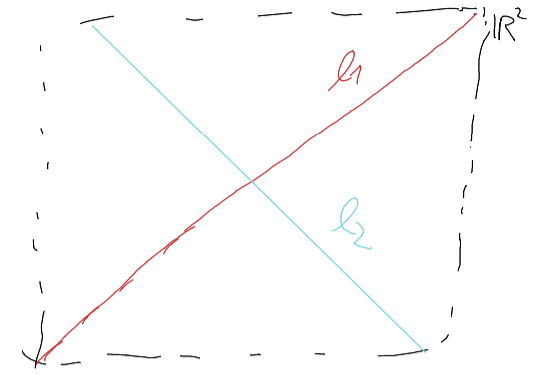
\includegraphics[width=.7\textwidth]{sketch_6_01.png}
    \caption{Sketch 6.01}
\end{figure}
\begin{figure}[H]
    \centering
    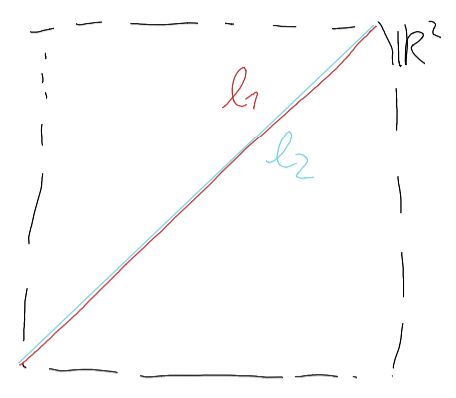
\includegraphics[width=.7\textwidth]{sketch_6_02.png}
    \caption{Sketch 6.02}
\end{figure}
\begin{figure}[H]
    \centering
    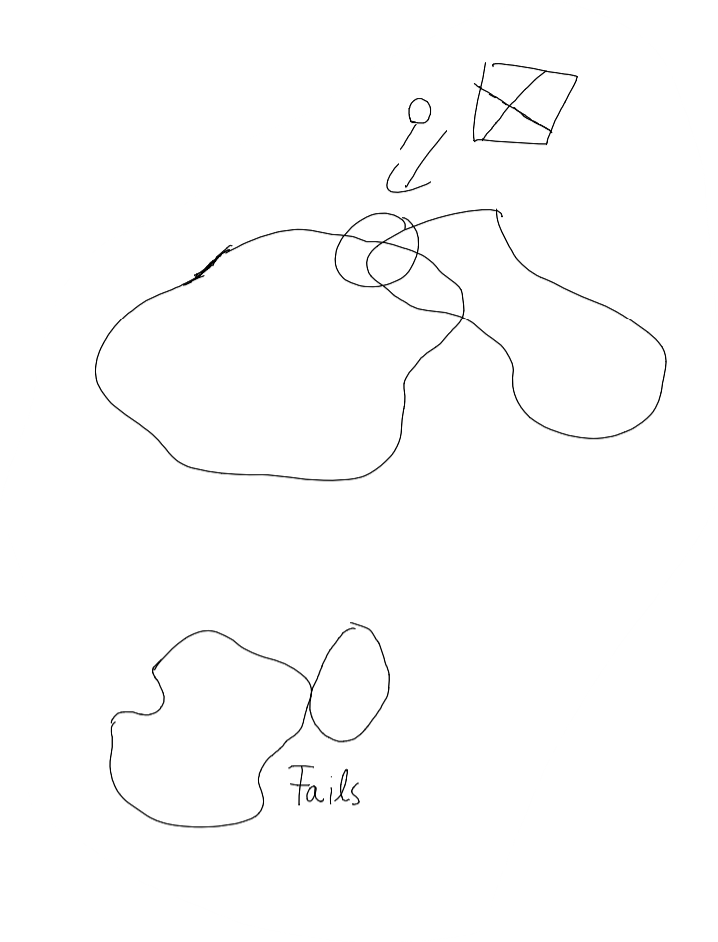
\includegraphics[width=.7\textwidth]{sketch_6_03.png}
    \caption{Sketch 6.03}
\end{figure}
\dhighlight{Observations:}
\begin{enumerate}
    \item transversality is stable (slight changes to the lines don't change transversality) \marginnote{Similarly to being full rank}
    \item transversality is generic(for pretty much any lines \(l_1,l_2\) they are transverse)
\end{enumerate}

One goal: Develop non-linear theory  of transversality. I.e. replace \(l_1,l_2\subset\R^2\) by manifolds.

Both of the above observations will still be true.  % sketches ...

\markeol{10}

\beginlecture{11}{15.11.2024}

\dhighlight{Announcement} On Tuesday, November 26, there will be a course evaluation. 

\begin{itemize}
    \item Please show up that day!
    \item Bring a phone / computer
\end{itemize}


Please add to your notes: %TODO: FIX
\begin{proof}[Proof of theorem \ref{thm:5.3}]
    \begin{figure}[H]
        \centering
        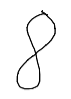
\includegraphics[width=.7\textwidth]{sketch_6_04.png}
        \caption{Sketch 6.04}
    \end{figure}
    
    Since \(S\hookrightarrow N\) is an embedding, \(i(U)\) is open in the 
    subspace topology, so there exists \(W\subset N\) such that \(i(U)=S\cap W\).

\end{proof}

\subsection{Transversality for submanifolds}

Let \(M\) be a smooth manifold. 
\begin{definition*}
    We say that a pair of submanifolds \(K,L\subset M\) are \dhighlight{transverse} at \(p\in K\cap L\) if 
    \marginnote{Here the sum is a gain the span of both of them}\[T_p K + T_p L = T_p M.\]
    We say that \(K,L\) are \dhighlight{transverse} and write \(K\pitchfork L\).
\end{definition*}

\begin{remark}
    In the literature, we  also see ``transversal'', ``transversally intersecting''. 
\end{remark}

\begin{example}
    \begin{figure}[H]
        \centering
        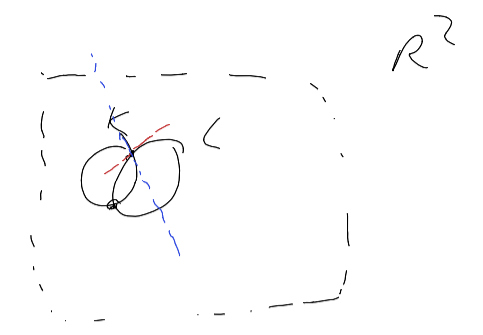
\includegraphics[width=.7\textwidth]{sketch_6_05.png}
        \caption{Sketch 6.05}
    \end{figure}
    \(K,L\) are transverse.
    \begin{figure}[H]
        \centering
        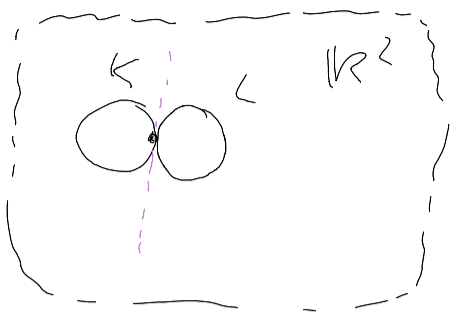
\includegraphics[width=.7\textwidth]{sketch_6_06.png}
        \caption{Sketch 6.06}
    \end{figure}
    \(T_p K=T_P L\), transversality fails.
\end{example}

\begin{lemma}\label{lem:6.1}\marginnote{Key lemma for transversality}
    Let \(K^k,L^l\) be submanifolds of \(M\). If \(K,L\) are transversal, then 
    \(K\cap L \subset M\) is a submanifold.
\end{lemma}

\begin{remark}
    In general, if \(S,T\) are submanifolds of \(N\), then \(S\cap T\) need not be a topological submanifold.
    For example: \(f:\R^2\to R\)
    \[f(x,y)=x^2-y^2.\]
    Let \(g:\R^2\to \R\) 
    \[g(x,y)=0.\]
    Let \(S=\{(x,y,z)\mid z=f(x,y)\}\subset \R^{2+1}\) and \(T=\{(x,y,z)\mid z=g(x,y)\}\subset \R^{2+1}\).
    But \[S\cap T=\{(x,y,z)\mid z=0,x^2-y^2=0\}\]
    \begin{figure}[H]
        \centering
        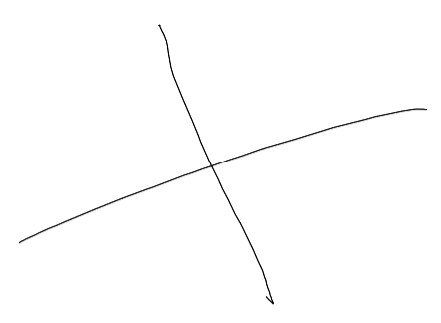
\includegraphics[width=.7\textwidth]{sketch_6_07.png}
        \caption{Sketch 6.07}
    \end{figure} 
    Look at the derivative at 0 .... % TODO
\end{remark}

\begin{proof}
    This is a local question, e.g. by theorem \ref{thm:5.3}. So we may as well assume that \(M=U\subset \R^n\).
    We can also assume that \(0\in U\).
    
    It is enough to check that \(K\cap L\) smooth submanifold in a neighborhood of \(p=0\). By rank theorem (\ref{thm:4.3}), we may assume 
    (after possibly further shrinking \(U\ni 0\)) that \(K=f^{-1}(0),f:U\to\R^{n-k}\),
    \(L=g^{-1}(0), g:U\to\R^{n-l}\) where \(f,g\) have full rank.

    \begin{figure}[H]
        \centering
        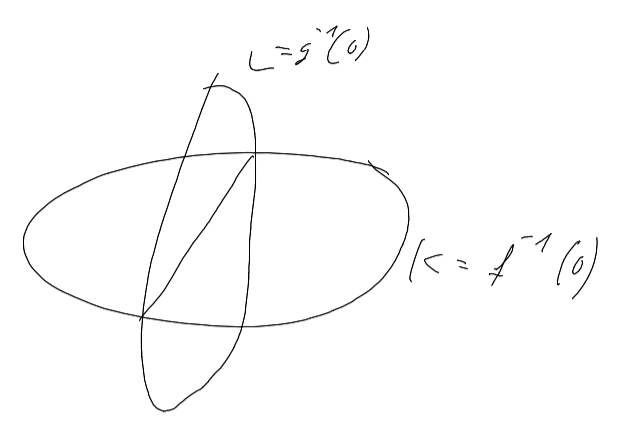
\includegraphics[width=.7\textwidth]{sketch_6_08.png}
        \caption{Sketch 6.08}
    \end{figure}
    Now we consider \(H=(f,g):U\to \R^{n-k}\oplus \R^{n-l}\). It is enough to prove that \(dH_0\) is 
    surjective (by the rank theorem). Note that \(H^{-1}(0)=f^{-1}(0)\cap g^{-1}(0)=K\cap L\).

    To see surjectivity of \(dH_0\), we consider the exact sequences: 
    \begin{figure}[H]
        \centering
        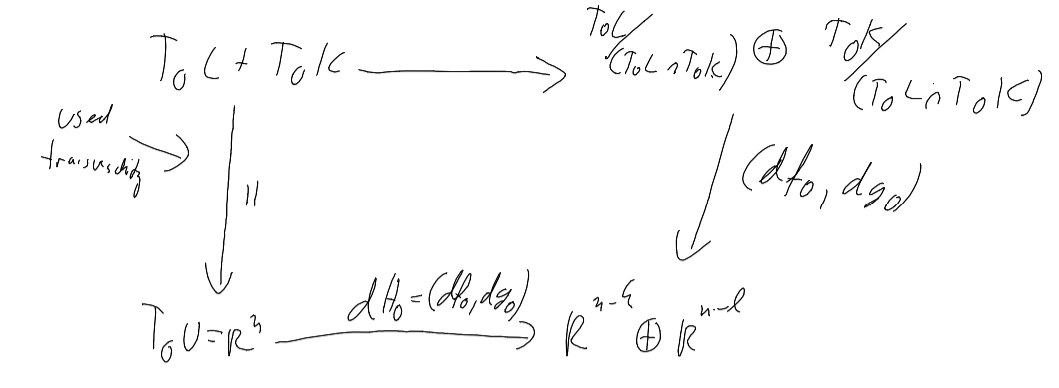
\includegraphics[width=.7\textwidth]{sketch_6_09.png}
        \caption{Sketch 6.09}
    \end{figure}
    The horizontal map \(T_0 L + T_0 K\to T_L/(T_0L\cap T_0K)\oplus T_K/(T_0L\cap T_0K)\) sends \(v+w\)
    to \((v,w)\). This is well defined, because if \(v+w=v'+w'\implies v-v'=w-w'\in T_0L\cap T_0K\). (Equivalently, this map is 
    just quotient by \(T_0L\cap T_0K\)) % TODO: FIX .?

    Clearly the R.H vertical arrow is injective: the kernel of \(df_0=T_0K\), so \((df_0)\restrict{T_0L/(T_0L\cap T_0K)}\) and similarly for \(dg_0\).
    To prove the R.H. vertical arrow is an isomorphism, do a dimension count:\marginnote{Exact sequence} 
    %TODO: FIX arrows
    \[0\to T_0K\cap T_0L\stackrel{v\mapsto (v,v)}{\to} T_0K + T_0L\stackrel{(u,w)\mapsto u-w}{\to} T_0U\equiv \R^n\to 0\]
    \(\implies \dim(T_0K\cap T_0L)+n=k+l\implies \dim(T_0L/_{(T_0K\cap T_0L)})=l-(k+l-n)=n-k\) and \(\dim(T_0K/_{(T_0K\cap T_0L)})=k-(k+l-n)=n-l\).
    We conclude that the R.H. vertical arrow is an isomorphism. 
\end{proof}

\begin{remark}
    We have 
    \begin{figure}[H]
        \centering
        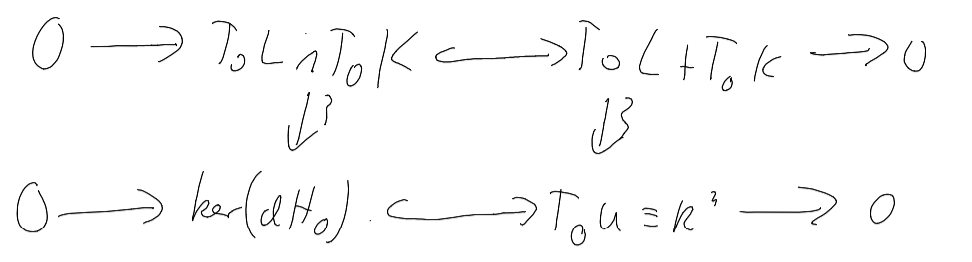
\includegraphics[width=.7\textwidth]{sketch_6_10.png}
        \caption{Sketch 6.10}
    \end{figure}
    where the left vertical arrow is an isomorphism, due to the 5'lemma or diagram chasing.

    Hence \(\ker (dH_0)=T_0L\cap T_0K=T_0(L\cap K)\).
\end{remark}

\subsection{Transversality of maps}

\begin{definition*} % TODO: FIX
    Let \begin{figure}[H]
        \centering
        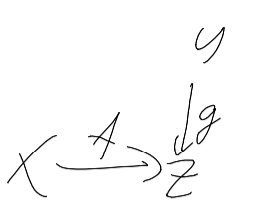
\includegraphics[width=.7\textwidth]{sketch_6_11.png}
        \caption{Sketch 6.11}
    \end{figure}
    be a diagram in Top (the category of topological spaces). We let \(X\substack{\times\\z} Y \coloneqq \{(x,y)\mid f(x)=g(y)\}\subset X\times Y\),
    endowed woth the subspace topology. We call \(X\substack{\times\\z} Y\) the \dhighlight{fiber product (of the diagram)}.
\end{definition*}

\begin{remark}[(for enthusiasts only)]
It can be shown that given any topological space \(W\in \text{Top}\) and maps 
\begin{figure}[H]
    \centering
    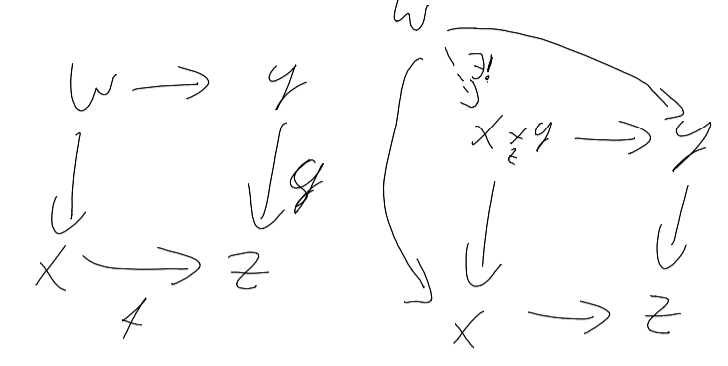
\includegraphics[width=.7\textwidth]{sketch_6_12.png}
    \caption{Sketch 6.12}
\end{figure}
there exists a unique map \(W\to X\substack{\times\\ z} Y\) commutes.(Universal property)
\end{remark}

Lots of categories admit fiber products! This is a good property for categories to have. 

\dhighlight{Bad news:} The (not-full) subcategory \(\maninf\subset\text{Top}\) does not admit 
fiber products (nor does \(\man0\subset\text{Top}\)). 
\begin{example}[Non-example]
    \(Z=\R^{2+1},X=\text{graph}(x^2-y^2),Y=\text{graph(0)}\).
\end{example} 

\begin{definition*}
    Let \begin{figure}[H]
        \centering
        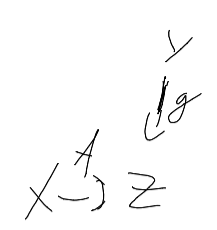
\includegraphics[width=.7\textwidth]{sketch_6_13.png}
        \caption{Sketch 6.13}
    \end{figure}
    be a diagram in \(\maninf\). We say that \(f,g\) are transverse at \(z=f(x)=g(y)\) if 
    \[\text{im }df_x+\text{im }dg_y=T_zZ.\]
    We say that \(f,g\) are \dhighlight{transverse} and say \(f\pitchfork g\) if this holds 
    for all such \(z\).
\end{definition*}

\begin{remark}
    Transversality for maps generalizes transversality for submanifolds. Take the diagram 
    \begin{figure}[H]
        \centering
        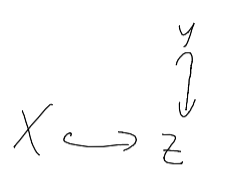
\includegraphics[width=.7\textwidth]{sketch_6_14.png}
        \caption{Sketch 6.14}
    \end{figure}
\end{remark}

\begin{proposition}\label{prop:6.2}
    If \(f\pitchfork g\), then \(X\substack{\times\\z} Y \stackrel{i}{\to} X\times Y\) is a smooth embedding.
\end{proposition}

\begin{figure}[H]
    \centering
    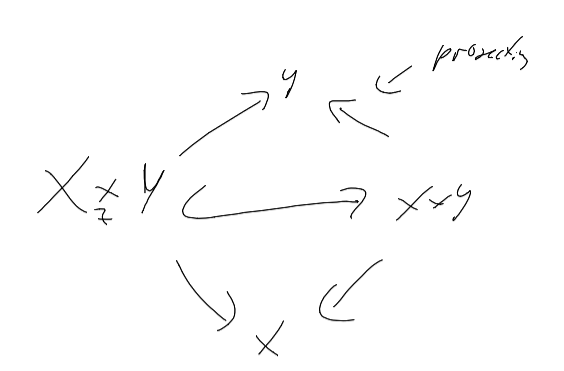
\includegraphics[width=.7\textwidth]{sketch_6_15.png}
    \caption{Sketch 6.15}
\end{figure}

\begin{proof}
    Some observations:
    \begin{itemize}
        \item exercise sheet 07: \(X\substack{\times\\z}X\times Y\) is proper.
        \item similarly to the proof of theorem \ref{thm:5.6:whithney}, it is enough to prove that 
              \(i\) is an injective immersion. By definition \(i\) is injective. Therefore we need to check that \(i\) is smooth and the differential is injective.
    \end{itemize}

    Consider 
    \begin{figure}[H]
        \centering
        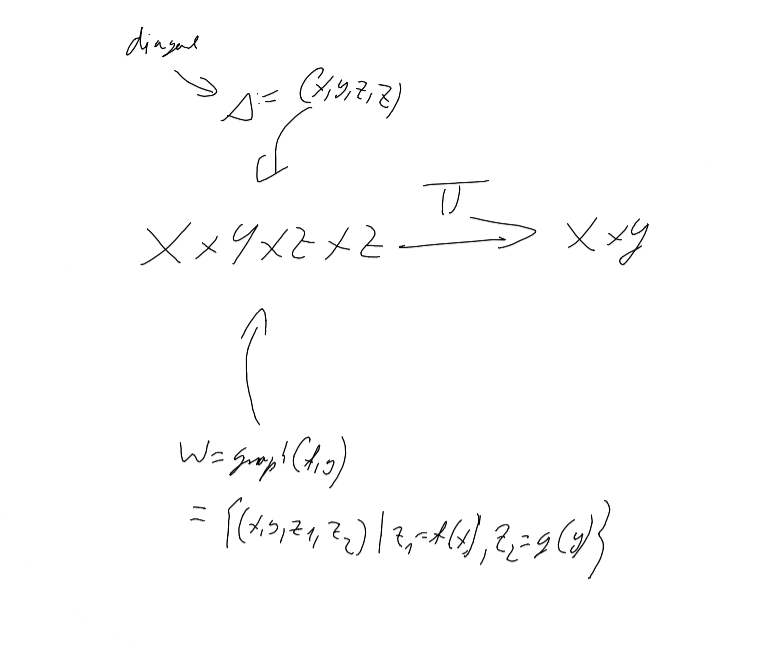
\includegraphics[width=.7\textwidth]{sketch_6_16.png}
        \caption{Sketch 6.16}
    \end{figure}
    Then \[W\cap \Delta=\{(x,y,z_1,z_2)\mid z_1=z_2=f(x)=g(y)\}=X\substack{\times\\z}Y.\]
    We have: 
    \begin{figure}[H]
        \centering
        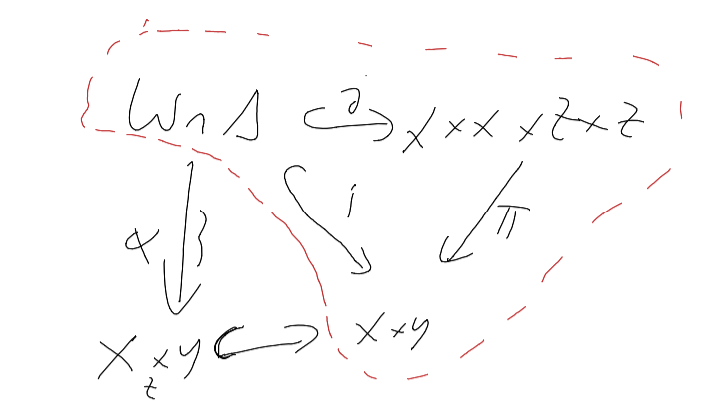
\includegraphics[width=.7\textwidth]{sketch_6_17.png}
        \caption{Sketch 6.17}
    \end{figure} 
    \(\alpha\) is clearly bijective and continuous. It is elementary that \(\alpha\) is a closed map.
    That means we have to check the limit points. \(W\cap \Delta\) is closed, i.e. contains the same limit points\dots   
    Therefore \(\alpha\) is a homeomorphism.

    By lemma \ref{lem:6.1}, if we can show that \(W\pitchfork \Delta\), then \(W\cap \Delta\stackrel{j}{X\times Y\times Z\times Z}\) is smooth embedding. 
    Hence \(i\coloneqq \pi\circ j\) smooth. Let us now check that \(W\pitchfork \Delta\) at some arbitrary point \(p=(x,y,z,z)\in W\cap \Delta\subset X\times Y\times Z\times Z\).
    Note that \(z=f(x)=g(y)\). We have \[T_pW=\{(v,w,df_x(v),dg_y(w))\}\]
    and 
    \[T_p\Delta=\{v',w',u,u\},\]
    where \(v,v'\in T_xX,w,w'\in T_yY,u\in T_zZ.\)
    We need to check: \(T_p W+T_p\Delta=T_p(X\times Y\times Z\times Z)\). We must show that for an arbitrary \((a,b,c,d)\in T_p(X\times Y\times Z\times Z)=T_XX\oplus T_yY\oplus T_zZ \oplus T_zZ,\)
    
    \markeol{11}
\end{proof}


